\documentclass[12pt,a4paper]{report}
\usepackage[pdftex]{graphicx}
\usepackage{styles}
\usepackage{url} 
\usepackage[bookmarks, colorlinks=false, pdfborder={0 0 0}, pdftitle={<pdf title here>}, pdfauthor={<author's name here>}, pdfsubject={<subject here>}, pdfkeywords={<keywords here>}]{hyperref} 
\usepackage{minted}
\usepackage{tikz}
\usepackage{colortbl}
\usepackage{hyperref}
\usepackage{textcomp}
\usepackage{amssymb}
\usetikzlibrary{matrix, arrows.meta, positioning, fit}
\usetikzlibrary{calc}
\begin{document}
\renewcommand\bibname{References} 
% concession

\begin{titlepage}

\begin{center}

\textup{\small {\bf Summer Internship Project} \\ Report}\\[0.3in]

% Title
\Large \textbf {\scol{\bf Formal verification of programs with pointers }}\\[0.7in]


       

% Submitted by
\normalsize Submitted by \\[0.2in]
\scol{\textbf{Oualid CHABANE}}\\
Third year of bachelor's double degree in \\ Computer Science, Magistère d'informatique track.\\
Faculty of sciences of Orsay, university of Paris-Saclay.

\vspace{.2in}
Under the guidance of\\[0.2in]
\scol{\textbf{Arnaud Goulfouse}}\\
\scol{\textbf{Paul Patault}}\\
\scol{\textbf{Jean-Christophe Filliâtre}}\\

\vspace{.3in}

% Bottom of the page
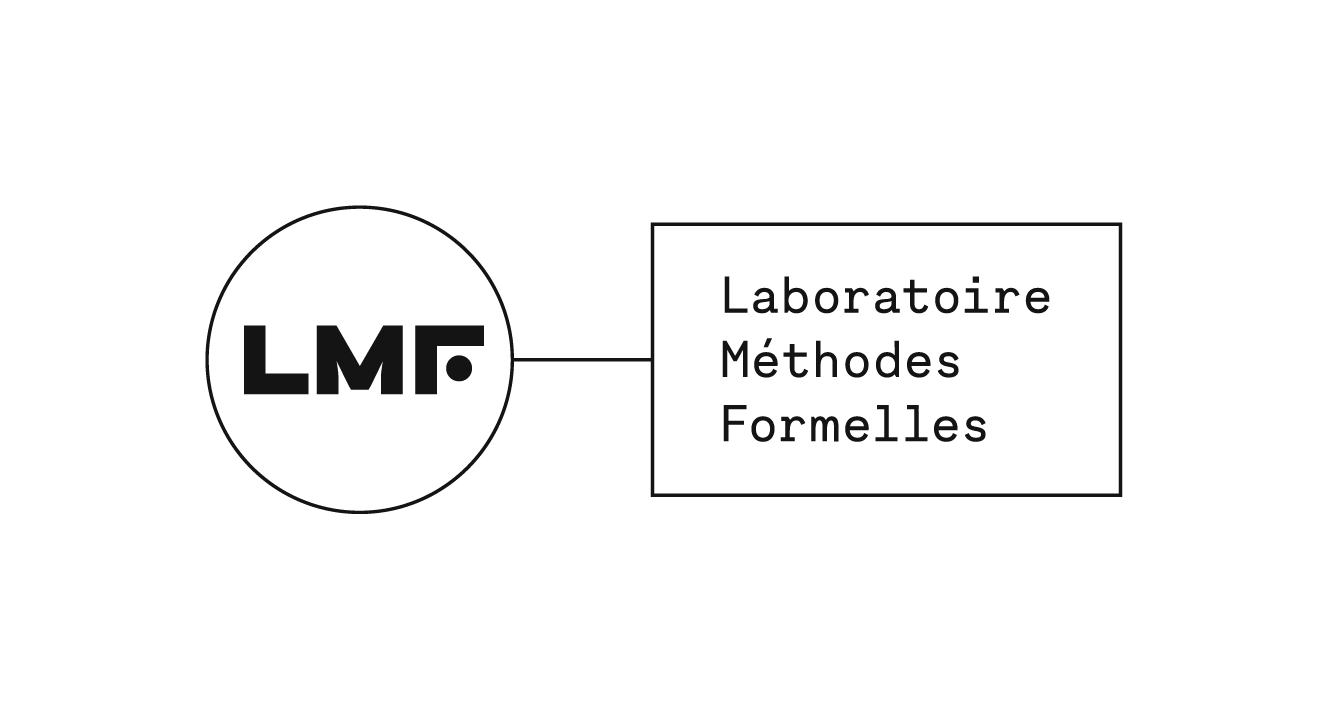
\includegraphics[width=0.5\textwidth]{lmf.png}\\[0.1in]
\Large{Department of Formal methods}\\
\normalsize
\textsc{ The Laboratoire Méthodes Formelles (LMF). }\\
4, avenue des Sciences, 91190 Gif-sur-Yvette \\
\vspace{0.2cm}
Summer Internship 2025

\end{center}

\end{titlepage}

% \input{abstract}

\pagenumbering{roman}
\tableofcontents


\newpage
\pagenumbering{arabic} 

\chapter{Introduction}

\section{\scol{The Laboratoire Méthodes Formelles (LMF)}}
LMF is a joint research centre of University Paris-Saclay, CNRS, ENS Paris-Saclay, Inria, and CentraleSupélec, it's divided to multiple departments interesting to various topics such as type systems, topology and quantum computing. My research project took place within \scol{Toccata's team} of the formal methods department. I worked on verification of programs with pointers under the supervision of \scol{Jean-Cristophe Filliâtre}, \scol{Arnaud GOLFOUSE} and \scol{Paul PATAULT}.
There are multiple verification tools widely used and developed at the LMF research center. Among these tools, we find Creusot, Why3, Coma and AltErgo. 

\section{\scol{Le langage de preuve Creusot}}
\textsc{Creusot} is a formal verification language used to verify \textsc{Rust} code. It checks the safety of code against compile-time and runtime panics, integer overflows, and, more importantly, the logical correctness of the code, ensuring it adheres to its specifications.\\
\textsc{Creusot} operates on top of \textsc{Why3} indirectly by translating Rust code into an intermediate verification language known as \textsc{Coma}. It facilitates the verification, and it also gives \textsc{Creusot} access to the full access to \textsc{Why3}'s features.
Below is a simple example of \textsc{Creusot} code that verifies the correctness of the \texttt{SUM} function.
\newpage
% \hypertarget{myanchor}{This is a custom anchor.}
% ...
% \hyperlink{myanchor}{Jump to custom anchor}

\begin{figure}[h]
  \centering
  \begin{minipage}{0.9\linewidth}
    \begin{minted}[linenos, fontsize=\small]{rust}
extern crate creusot_contracts;
use creusot_contracts::*;

#[requires(n@ * (n@ + 1) / 2 < u32::MAX@)]
#[ensures(result@ == n@ * (n@ + 1) / 2)]
pub fn sum_first_n(n: u32) -> u32 {
    let mut sum = 0;
    #[invariant(sum@ * 2 == produced.len() * (produced.len() + 1))]
    for i in 1..=n {
        sum += i;
    }
    sum
}
    \end{minted}
   \caption{A Rust function verified with \textsc{Creusot} to compute the sum of the first \texttt{n} natural numbers.}
    \label{fig:sum-first-n}
  \end{minipage}
\end{figure}

\textbf{Explication}: 

The function \textsc{sum\_first\_n} shown above computes the sum of the first \texttt{n} natural numbers. The expressions highlighted in yellow represent its specification:
\begin{itemize}
  \item \textbf{Precondition:} It asserts that the sum of the first \texttt{n} natural numbers where \texttt{n} is provided as a parameter,  does not overflow the capacity of the result type. This ensures that the final sum, which will be stored in the return variable will not exceed the capacity of the return type.
  
  \item \textbf{Postcondition:} It states that the returned result is equal to the expected mathematical value: \texttt{n * (n + 1) / 2}
  
    \item \textbf{Loop invariant:} The expression \texttt{produced.len()} corresponds to the number of iterations performed so far, it effectively can play the role of the loop index by applying a transformation. The reason we cannot refer directly to the loop index is due to scoping limitations.
\end{itemize}


Recently, ghost code has been introduced to \textsc{Creusot}. The subtlety lies in the fact that ghost code is separate from the original code, therefore, it can be erased safely after compile-time which allows to execute only the original code and the corresponding logical formulas which is faster and safer to prove code. Below are some examples of how to write ghost code in \textsc{Creusot}.

%grace au code ghost on peut tirer des principes de la log de sép vers le monde logique,  PARLER SUR LE TYPAGE...disjoint_lemma, faut iclure dans  la partie ghost une explicaiton sur pour quoi la spec de disjoint_lemma ne peut pas marcher si c'était une fonciton logique....

\hypertarget{ghostcode}{This is the target text.}
Another subtle aspect of ghost code is its capacity to drag separation logic principles which are implicitly guaranteed by the \texttt{Rust} type system into the logical world. To be more precise, let us consider the interface of \texttt{PtrOwn<T>::disjoint\_lemma} as an illustrative example.

\begin{figure}[h]
  \centering
  \begin{minted}[linenos, fontsize=\small]{rust}
/// If one owns two PtrOwns in ghost code, then they are for different pointers.
#[ghost]
#[ensures(own1.ptr().addr_logic() != own2.ptr().addr_logic())]
#[ensures(*own1 == ^own1)]
pub fn disjoint_lemma(own1: &mut PtrOwn<T>, own2: &PtrOwn<T>)
  \end{minted}
  \caption{\texttt{PtrOwn<T>::disjoint\_lemma} contract}
  \label{fig:disjoint-lemma}
\end{figure}

\ccomp{EXPLAIN MORE}

% ETAT DE LART
\chapter{State of art}
\section{\scol{Reynolds article}}

Reynolds' article introduced a new concept in formal program verification: \emph{Separation Logic}, an extension of Hoare Logic that facilitates automatic proofs on low-level imperative programs that use shared mutable data structures, by reasoning about disjoint parts of the heap. It greatly simplifies the formalization and verification of many problems that are otherwise difficult to handle using traditional Hoare Logic, such as concurrency, memory management, and aliasing.

% \hypertarget{myanchor}{This is the target text.}

% You can jump to it using \hyperlink{myanchor}{this link}.

\textsc{Creusot} does not support Separation Logic, its principles can be emulated through the use of the \textsc{Rust} type system and ghost code, as \hyperlink{ghostcode}{previously discussed$\dagger$}. There are, however, more specialized tools designed specifically for reasoning with Separation Logic. One such tool is \textsc{Viper}, a Rust verifier that supports Separation Logic. It is built on top of \textsc{Boogie}, an intermediate verification language (IVL) developed by Microsoft Research, and is widely used in the field of formal verification. The illustration below clarifies the relationships between these languages and their connection to Separation Logic.

\ccomp{give examples of Creusot where we can implement the separation logic, and compare with boogie or viper}
\newpage
\vspace{1cm}
\begin{figure}[h]
  \centering
    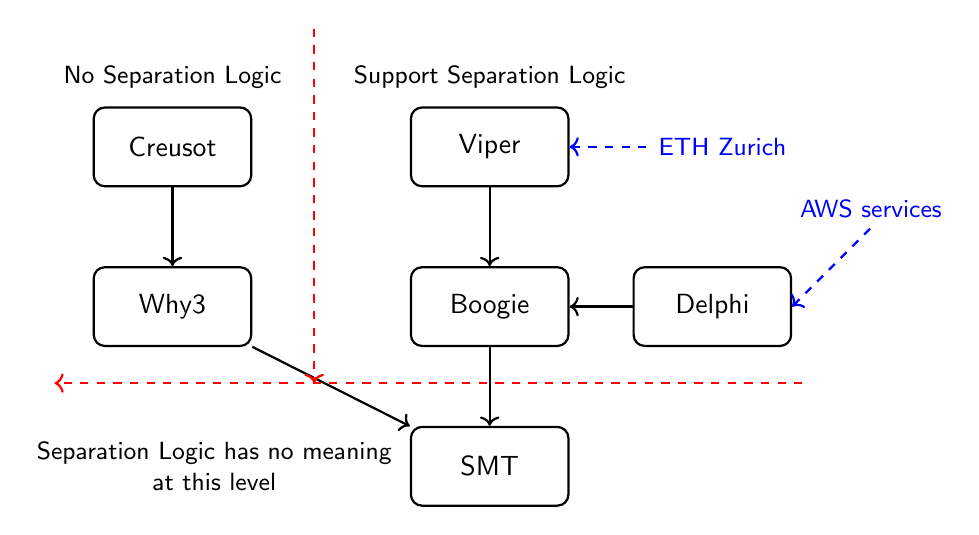
\begin{tikzpicture}[
      node distance=1cm and 2cm,
      every node/.style={font=\sffamily},
      box/.style={draw, rectangle, rounded corners, minimum width=2cm, minimum height=1cm, align=center},
      ->, thick
    ]
    
    
    % Nodes
    \node[box] (creusot) {Creusot};
    \node[box, right=of creusot] (viper) {Viper};
    \node[box, below=of viper] (boogie) {Boogie};
    \node[box, left=of boogie] (why3) {Why3};
    \node[box, below=of boogie] (smt) {SMT};
    \node[box, right=0.8cm of boogie] (delphi) {Delphi};
    
    % Arrows
    \draw (creusot) -- (why3);
    \draw (viper) -- (boogie);
    \draw (why3) -- (smt);
    \draw (boogie) -- (smt);
    \draw (delphi) -- (boogie);
    
    % Add dashed vertical separation line
    \draw[dashed, red, line width=0.8pt] 
      (1.8,1.5) -- (1.8,-3);
    \draw[dashed, red, line width=0.8pt] 
      (8,-3) -- (-1.5,-3);
    % Arrow pointing to Delphi
    \draw[<-, dashed, blue] (delphi.east) -- ++(1,1) node[above, font=\small\sffamily, blue] {AWS services};
    \draw[<-, dashed, blue] (viper.east) -- ++(1,0) node[right, font=\small\sffamily, blue] {ETH Zurich};
    
    % Add explanatory labels
    \node[above=0.1cm of creusot, align=center, font=\small\sffamily] (leftlabel) 
      {No Separation Logic};
    \node[above=0.1cm of viper, align=center, font=\small\sffamily] (rightlabel) 
      {Support Separation Logic};
    \node[left=0.1cm of smt, align=center, font=\small\sffamily] (rightlabel) 
      {Separation Logic has no meaning\\ at this level};
    \end{tikzpicture}
  \vspace{0.5cm}
  \caption{Illustration of the relationship between verification tools and intermediate languages.}
  \label{fig:verification-diagram}
\end{figure}

To prove properties of algorithms on data structures, it's usually not enough to rely only on the program's representation. We often build a logical model of the data and connect it to the program state using predicates. It's better if the logical model is inductive, because provers generally work better with inductive data structures, for instance, the intuitive logical modeling of lists are sequences, therefore we can write the following predicate to represent a list:

\begin{center}
\begin{tabular}{l}
\texttt{list $\epsilon$ i = i = nil} \\
\texttt{list (a.$\alpha$) i = $\exists$j, list $\alpha$ j $\land$ i $\hookrightarrow$ a}
\end{tabular}
\end{center}
\texttt{i $\hookrightarrow$ a} means \texttt{i} points to \texttt{a}

\section{\scol{Different ways of implementing the problem}}
The list reversal problem has already been proven in two different ways in \textsc{Creusot}, but both methods have certain limitations:

\begin{itemize}
\item \textbf{\textsc{BOX} method}: This approach models lists using \texttt{Rust Box} type. However, it imposes strong restrictions on the memory model by prohibiting any form of sharing or aliasing, since \texttt{Box} does not support multiple references to the same memory location.
\item \textbf{Memory model method}: This approach consists of passing an object that models the entire memory as a parameter to each method to be verified, therefore, proving requires reasoning over the complete memory state. However, this approach prevents \ccomp{...todo}.
\end{itemize}

% PROBLEM DEFINITION AND SOLUTION
\chapter{Problem definition and proposed solution}

\section{Problem definition}
\section{Proposed solution}

\begin{figure}[h]
  \centering
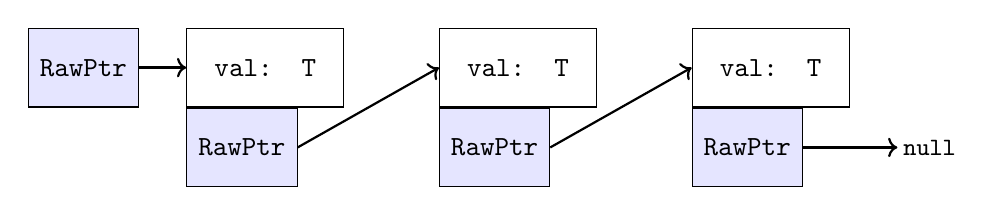
\begin{tikzpicture}[
  ptr/.style={draw, rectangle, minimum width=1.4cm, minimum height=1cm, font=\ttfamily, fill=blue!10, inner sep=4pt},
  innerbox/.style={draw, rectangle, minimum width=1.4cm, minimum height=1cm, font=\ttfamily, inner sep=10pt},
  arrow/.style={->, thick},
  every node/.style={inner sep=2pt}
]

% First RawPtr
\node[ptr, anchor=north west] (p1) {RawPtr};

% First Node (two fields)
\node[innerbox, right=0.6cm of p1.north east, anchor=north west] (n1val) {val: T};
\node[ptr, below=0pt of n1val.south west, anchor=north west] (n1ptr) {RawPtr};
% Second Node (two fields)
\node[innerbox, right=1.2cm of n1val.north east, anchor=north west] (n2val) {val: T};
\node[ptr, below=0pt of n2val.south west, anchor=north west] (n2ptr) {RawPtr};

% Third Node (two fields)
\node[innerbox, right=1.2cm of n2val.north east, anchor=north west] (n3val) {val: T};
\node[ptr, below=0pt of n3val.south west, anchor=north west] (n3ptr) {RawPtr};

% Null node
\node[font=\ttfamily\small, right=1.2cm of n3ptr] (nullnode) {null};

% Arrows between elements
\draw[arrow] (p1.east) -- (n1val.west);
\draw[arrow] (n1ptr.east) -- (n2val.west);
\draw[arrow] (n2ptr.east) -- (n3val.west);
\draw[arrow] (n3ptr.east) -- (nullnode.west);

\end{tikzpicture}


  \caption{Representation of the list in program world.}
  \label{fig:rawptr-list}
\end{figure}


\begin{figure}[h]
  \centering

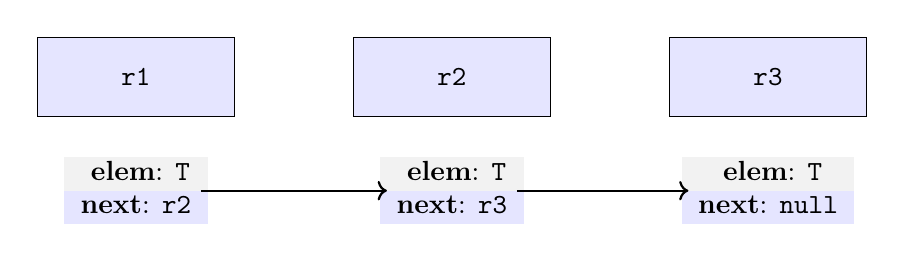
\begin{tikzpicture}[
  ptr/.style={fill=blue!10, draw, minimum width=2.5cm, minimum height=1cm, font=\ttfamily},
  node/.style={draw, minimum width=2.5cm, minimum height=2cm, font=\ttfamily, align=center},
  arrow/.style={->, thick}
]

\matrix (nodes) [matrix of nodes, column sep=1.5cm, row sep=0.4cm, nodes={anchor=center}] {
  |[ptr]| \texttt{r1} & |[ptr]| \texttt{r2} & |[ptr]| \texttt{r3} \\
  % Nodes with two stacked fields
  \begin{tabular}{@{}c@{}}
    \cellcolor{gray!10} \textbf{elem}: \texttt{T} \\
    \cellcolor{blue!10}\textbf{next}: \texttt{r2}
  \end{tabular}
  &
  \begin{tabular}{@{}c@{}}
    \cellcolor{gray!10} \textbf{elem}: \texttt{T} \\
    \cellcolor{blue!10}\textbf{next}: \texttt{r3}
  \end{tabular}
  &
  \begin{tabular}{@{}c@{}}
    \cellcolor{gray!10} \textbf{elem}: \texttt{T} \\
    \cellcolor{blue!10}\textbf{next}: \texttt{null}
  \end{tabular}
  \\
};

% Arrows
\draw[arrow] (nodes-2-1.east) -- (nodes-2-2.west);
\draw[arrow] (nodes-2-2.east) -- (nodes-2-3.west);

\end{tikzpicture}

  \caption{Representation of the list in the logical world.}
  \label{fig:rawptr-list}
\end{figure}

% Conclusion and prespectives
\chapter{Conclusion and prespectives}

\section{Appendix}

\hypertarget{reversal}{\subsection{\scol{\texttt{in\_place\_reversal} algorithm}}}
\begin{align*}
&\texttt{j := nil; while i } \texttt{<>} \texttt{ nil do} \\
&\quad \quad \texttt{(k := [i + 1]; [i + 1] := j; j := i; i := k).}
\end{align*}
\subsection{\scol{Code}}
\begin{minted}[breaklines=true]{rust}
extern crate creusot_contracts;
use ::std::ptr;
use creusot_contracts::ptr_own::{PtrOwn, RawPtr};
use creusot_contracts::*;
pub struct Node<T> {
    elem: T,
    pub next: RawPtr<Node<T>>,
}

impl<T> Node<T> {
    #[predicate]
    #[variant(perm_seq.len())]
    fn list(l: RawPtr<Self>, perm_seq: Seq<PtrOwn<Node<T>>>) -> bool {
        pearlite! {
            if l.is_null_logic() {
                perm_seq.len() == 0
            } else {
                 if perm_seq.len() > 0 {
                    let ptr = perm_seq[0].ptr();
                    l == ptr && Self::list(perm_seq[0].val().next, perm_seq.tail())
                } else {
                    false
                }
            }
        }
    }

    #[ensures(Self::list(result.0, *result.1))]
    #[ensures(result.0.is_null_logic())]
    pub fn empty() -> (RawPtr<Self>, Ghost<Seq<PtrOwn<Node<T>>>>) {
        (ptr::null(), Seq::new())
    }

    #[requires(Self::list(l, **seq))]
    #[ensures(Self::list(result,  *^seq))]
    #[ensures(forall<i:Int> 0 <= i && i < (^seq).tail().len() ==> seq[i] == (^seq).tail()[i])]
    #[ensures((^seq)[0].val().elem == e)]
    #[ensures((^seq)[0].ptr() == result)]
    #[ensures((^seq).len() == seq.len() + 1)]
    pub fn cons(e: T, l: RawPtr<Self>, seq: &mut Ghost<Seq<PtrOwn<Node<T>>>>) -> RawPtr<Self> {
        let (raw, own) = PtrOwn::new(Node { elem: e, next: l });

        let _seq2 = snapshot!(**seq);
        ghost!(seq.push_front_ghost(own.into_inner()));
        proof_assert!(*_seq2 == seq.tail());

        raw
    }

    #[requires(Self::list(p, **seq))]
    #[requires(0 <= nth@ && nth@ < seq.len() )]
    #[ensures(seq[nth@].val().elem == *result)]
    pub fn nth(mut p: RawPtr<Self>, nth: i128, seq: &Ghost<Seq<PtrOwn<Node<T>>>>) -> &T {
        let mut i = 0;
        proof_assert!(**seq == seq.subsequence(0, seq.len()));
        #[invariant(0 <= i@ && i@ <= nth@)]
        #[invariant(Self::list(p, seq.subsequence(i@, seq.len())))]
        loop {
            let rw = unsafe {
                PtrOwn::as_ref(p, ghost!(seq.get_ghost(Int::new(i).into_inner()).unwrap()))
            };

            if i == nth {
                return &rw.elem;
            }

            p = rw.next;
            proof_assert!(seq.subsequence(i@, seq.len()).tail() == seq.subsequence(i@+1, seq.len()));
            i += 1;
        }
    }

    #[predicate]
    pub fn inverse(seq: Seq<PtrOwn<Node<T>>>, other: Seq<PtrOwn<Node<T>>>, lb: Int, lh: Int) -> bool
    where
        T: Sized,
    {
        pearlite! {
             forall<i: Int>
            lb <= i && i < lh
            ==> seq[i].val().elem == other[other.len() - i - 1].val().elem
        }
    }

    #[requires(Self::list(p, **seq))]
    #[ensures(Self::list(result, *^seq))]
    #[ensures(seq.len() == (^seq).len())]
    #[ensures(Self::inverse(**seq, *^seq, 0, (*^seq).len()))]
    pub fn reverse_in_place(
        mut p: RawPtr<Self>,
        seq: &mut Ghost<Seq<PtrOwn<Node<T>>>>,
    ) -> RawPtr<Self> {
        snapshot! {
            let _ = Seq::<T>::ext_eq;
        };
        let mut q: *const Node<T> = ptr::null();
        let mut reverted_seq = Seq::new();
        let _seq0 = snapshot!(**seq);

        #[invariant(Self::list(q, *reverted_seq))]
        #[invariant(Self::list(p, **seq))]
        #[invariant(Self::inverse(_seq0.subsequence(0, reverted_seq.len()), *reverted_seq, 0, reverted_seq.len()))]
        #[invariant(reverted_seq.len() + seq.len() == _seq0.len())]
        #[invariant(**seq == _seq0.subsequence(reverted_seq.len(), _seq0.len()))]
        #[invariant(inv(seq))]
        #[invariant(inv(reverted_seq))]
        while !p.is_null() {
            let _sloop_entry = snapshot!(**seq);
            let _revs_loop_entry = snapshot!(*reverted_seq);
            let p2 =
                unsafe { PtrOwn::as_mut(p, ghost!(seq.get_mut_ghost(*ghost!(0int)).unwrap())) };
            let next = p2.next;
            p2.next = q;
            q = p;
            p = next;
            let _sloop_exit = snapshot!(**seq);

            ghost!((*reverted_seq).push_front_ghost(seq.pop_front_ghost().unwrap()));

            //a0156: Assertion used to prove invariant #1 (we can remove it and use use_th seq.FreeMonoid instead)
            proof_assert!(reverted_seq.tail() == *_revs_loop_entry);

            //Hypothesis: invariant(Self::list (p, **seq))
            // We need to add to the hypothesis the fac that the tail of the previous seq is the new seq
            //a1369
            proof_assert!((*_sloop_exit).tail() == **seq);

            //In order to proof the last assertion, we need the following assertion
            //It esnures that seq.tail() didn't change between the beginig of the loop and the end, what ensures the stability of our invariant
            //a7070
            proof_assert!((*_sloop_exit).tail() == (*_sloop_entry).tail());

            //this should be enough to prove #[invariant(Self::list (p, **seq))], whith using the latter, creusot proves well the remaining invariant about q
            //proof_assert!(Self::list(p, (*snap2).tail()));
            //a1313
            proof_assert!(Self::list(p, (*_sloop_exit).tail()));
            // ==> invariant #1 checks for iteration n+1
        }
        //Pour montrer ensures#1 (ensures(seq.len() == (^seq).len() && Self::inverse(**seq, *^seq, 0, seq.len())))
        //a4224
        proof_assert!(_seq0.subsequence(0, reverted_seq.len()) == *_seq0);
        ghost!(**seq = reverted_seq.into_inner());
        q
    }
}

#[ensures(Node::list(result.0, *result.1))]
#[ensures(result.1.len() == vec.view().len())]
#[ensures(forall<i: Int> 0 <= i && i < vec.view().len() ==> (*result.1)[i].val().elem == vec.view()[i])]
pub fn list_of_vector1<T>(mut vec: Vec<T>) -> (RawPtr<Node<T>>, Ghost<Seq<PtrOwn<Node<T>>>>) {
    //Takes possession of elements in the vector
    let (mut l, mut seq) = Node::empty();
    let _vec0 = snapshot!(vec);
    #[invariant(forall<i: Int>
        vec.view().len() <= i && i < _vec0.view().len() ==> seq[i - vec.view().len()].val().elem == _vec0.view()[i])]
    #[invariant(Node::list(l, *seq))]
    #[invariant(vec.view().len() + seq.len() == _vec0.view().len())]
    #[invariant(forall<i: Int> 0 <= i && i < vec.view().len() ==> vec.view()[i] == _vec0.view()[i])]
    #[invariant(inv(seq))]
    loop {
        if let Some(v) = vec.pop() {
            l = Node::cons(v, l, &mut seq);
        } else {
            break;
        }
    }
    (l, seq)
}

pub fn tr() {
    let v1 = creusot_contracts::vec![1, 5, 3];
    let (list1, mut _seq1) = list_of_vector1(v1.clone());
    assert!(*Node::nth(list1, 0, &_seq1) == 1);
    assert!(*Node::nth(list1, 1, &_seq1) == 5);
    assert!(*Node::nth(list1, 2, &_seq1) == 3);
    let l2 = Node::reverse_in_place(list1, &mut _seq1);
    assert!(*Node::nth(l2, 2, &_seq1) == 1);
    assert!(*Node::nth(l2, 1, &_seq1) == 5);
    assert!(*Node::nth(l2, 0, &_seq1) == 3);

    print!("ok");
}
\end{minted}


\end{document}
